\chapter{Analysis}
%%%%%%%%%%%%%%%%%%%%%%%%%%%%%%%%%%%
%%%    PROJECT SPECIFICATION    %%%
%%%%%%%%%%%%%%%%%%%%%%%%%%%%%%%%%%%
 \section{Research Conclusions}
 \label{sec:analysis:researchConclusions}
  \begin{itemize}
   \item \textbf{Methodology}\\
    This project will make use of the Waterfall Model but with some changes regarding the documentation and some changes to some stages. In short there will be: no feasibility study, a prototype for hardware communication during the analysis, a few test classes during the design stage needed to be written to determine how some libraries work, a module documentation. The testing will be done after the full implementation is done. The project report will be written along with the project in parallel to the stages.
   \item \textbf{Chosen Hardware}\\
    The chosen technology is RFID based. The hardware that will be used are three OpenBeacon nodes and two CCC Sputnik tags. Three nodes to trilaterate a position and two tags so that collision can be tested.
   \item \textbf{Operating system}\\
    The main operating system for this project will be Linux. It will be used by the developer to develop the project and the project itself will only be tested on Linux.
   \item \textbf{License}\\
    The whole code will be licensed under the GPL.
   \item \textbf{Programming language and libraries}\\
    The primary programming language will be C++ in combination with the Qt library. The Qt library will support C++ on some core features like networking and string handling as well as on the GUI. For the web-interfaces PHP will be used.
   \item \textbf{Code version control system}\\
    To enable the ability for reverting code and have a save position if anything happens to the local code, the project will also be stored on a SVN server.
   \item \textbf{Build environment}\\
    For a quicker way to build the modules of each project CMake will be used. CMake supports the building process with automatic search for libraries, and linking them if needed to the binary.
   \item \textbf{Software Project Management System}\\
    Trac will be used for the project management. It provides easy web access to the subversion repository and has also a system, which supports some basic project management like a ticket system for the bug tracking. It also has a system for displaying the current state of the project and upcoming milestones and other functionalities to support the development.
   \item \textbf{Database}\\
    The database which will be used to support some modules of this project will be the MySQL database. It is well integrated in PHP, and for open source projects there is no fee to pay.
   \item \textbf{IPC}\\
    The IPC this project is using is mainly the D-Bus system. The network communication interfaces will be developed with a SSL (Secure Sockets Layer) based socket implementation, because the D-Bus support for network based IPC is still in development and does not work very well. It also lacks in security, so for the network communication a socket based SSL connection will be used.
  \end{itemize}

 \section{Project overview}
  \label{sec:analysis:ProjecSpec}
  The system needs to be split up into three layers (see figure \ref{fg:analysis:systemLayers}).
  \begin{figure}[h]
   \centering
   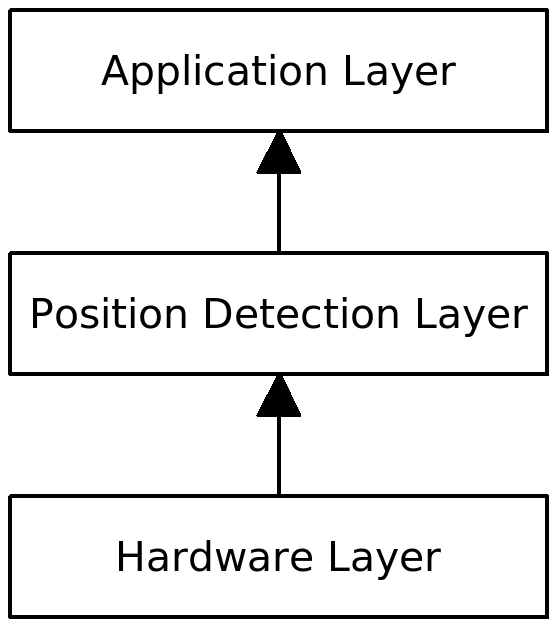
\includegraphics[scale=0.4]{Diagrams/systemLayers.png}
   \caption{Layers of the system}
   \label{fg:analysis:systemLayers}
  \end{figure}
  \begin{itemize}
   \item The hardware layer:\\
    This layer is communicating with the hardware.
   \item The position detection layer:\\
    This layer does all the objectives regarding the position detection.
   \item The application layer:\\
    This layer holds all the end user applications that are using the positions of the tags.
  \end{itemize}
  The advantages of this three layer system are that on one hand the different logics of the system are divided from each other and on the other hand each layer can be expanded with functionalities on its own. The hardware layer could be extended to support different types of hardware. The position layer could be extended by a calculation for a 3D position detection. And on the application layer a lot of different applications can be implemented to support a wide set of uses for the position detection system.

%%%%%%%%%%%%%%%%%%%%%%%%%%%%%%%%%%%%%%
%%%    GENERAL SYSTEM TEST PLAN    %%%
%%%%%%%%%%%%%%%%%%%%%%%%%%%%%%%%%%%%%%
 \section{General system test plan}
  \label{sec:analysis:generalSystemTestPlan}
  This section will not provide the detailed description about the single tests that have to be done. But it will describe what tests in general shall be done and how they shall be accomplished.

  \begin{itemize}
   \item Each layer shall be tested for its own, if it is working as it is meant to be.
   \item Each layer shall be checked upon the data it provides and if this data is appropriate.
   \item The data-flow between the layers shall be watched if there is some inconsistency.
   \item Data stored persistent shall be checked if it is stored in a proper way and not malformed.
   \item Every application with user input, shall be tested for the correctness of the error messages if the input is not as expected.
   \item If input derives from the Hardware it shall be checked if it is correct.
   \item Testing the whole system with all its applications and hardware.
  \end{itemize}
